\begin{figure}[htbp]
\begin{center}
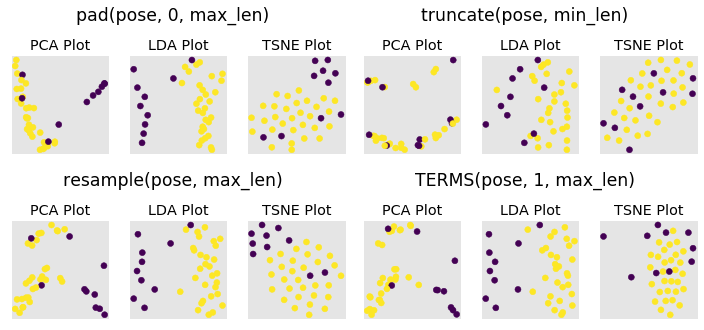
\includegraphics[width=12cm]{images/pre_processing_results.png}
\end{center}
\caption{Visualization of the effects of each method on a subset of  data used in this paper. Yellow indicates successful jump sequences and purple indicates unsuccessful jump sequences. Principle Component Analysis(PCA), Lindear Discriminant Analysis(LDA), t-Distributed Stochastic Neighbor Embedding (TSNE) are used to reduce the dimensionality to 2. It is worth noting that truncation severely impairs discriminating power because unsuccessful jumps are defined by a failure to land. Truncating the end of the sequence may discard this information.}
\label{figure:pre_processing_results}
\end{figure}
